\subsection{An example: the trefoil knot as a process}
The above intuitions are illustrated with an example, showing one way to
represent the trefoil knot as a process. Following the schema above,
the process encoding of the trefoil knot is a parallel composition of
three crossing circuits with a wiring harness whose design ensures that the
crossing circuits are connected to each other in a way that respects
the knot diagram. Additionally, we make each synchronization channel
local to each crossing via a restriction on that channel.

\begin{figure}[tbp]
\begin{center}
{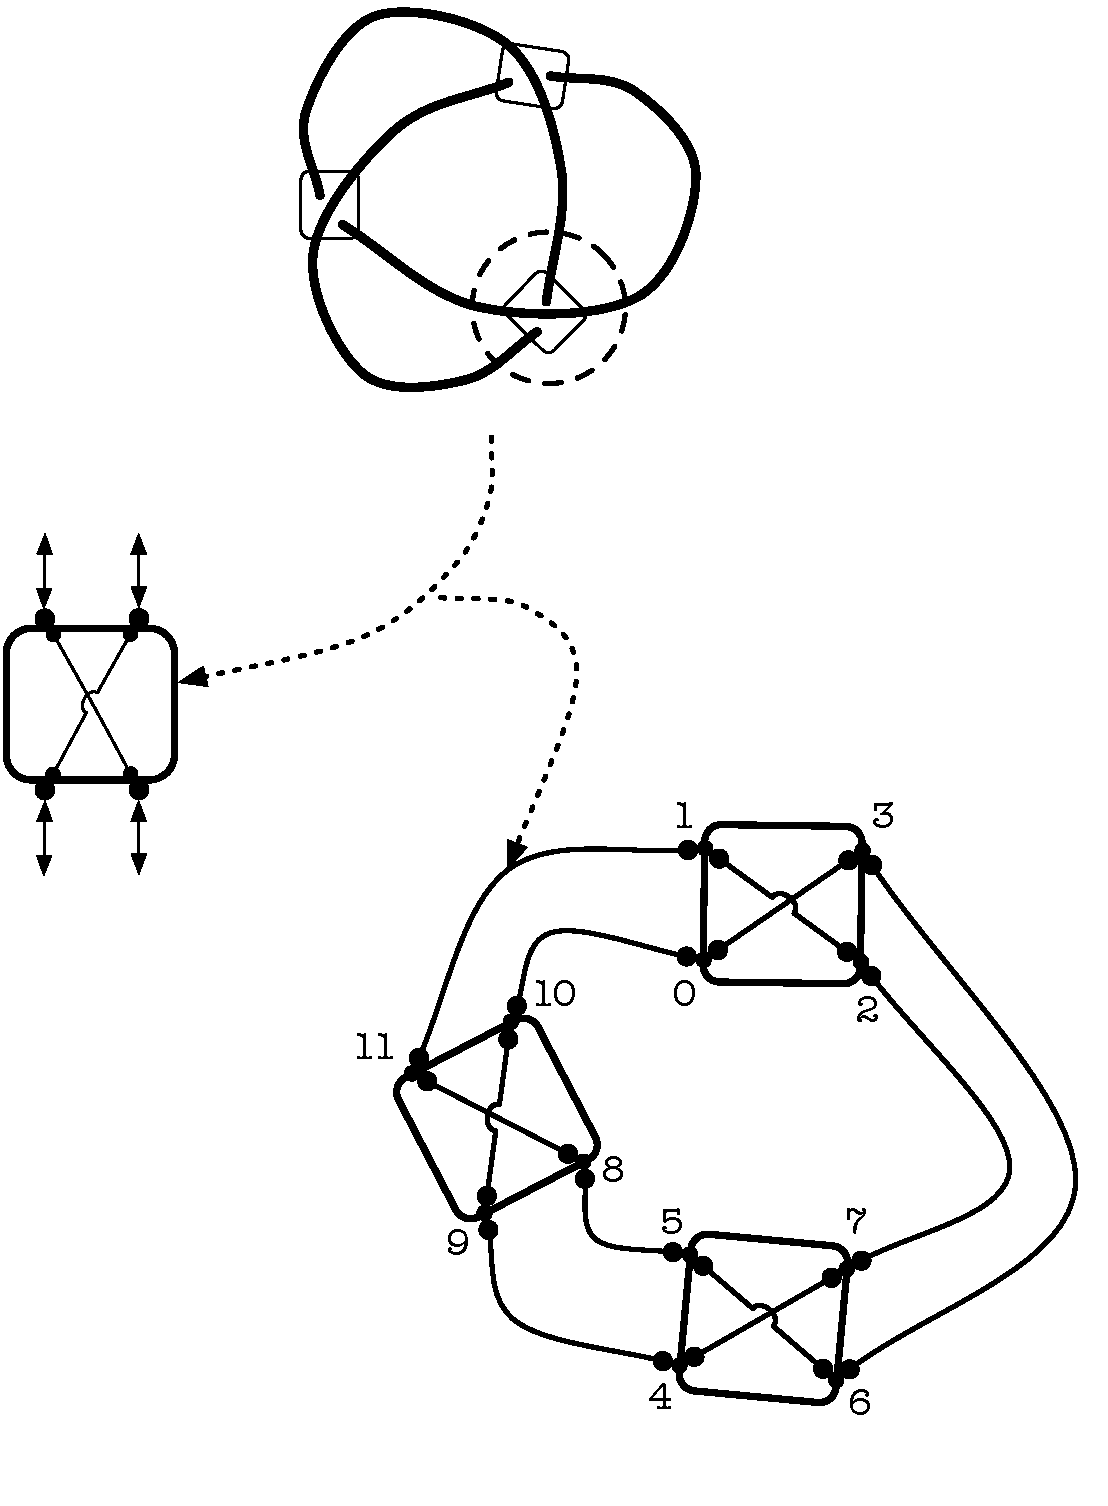
\includegraphics[width=3in]{../../illustrations/TrefoilMethodIllustration.pdf}}
\caption{ The $3_1$ (trefoil) knot as process. The ports in the
  circuit diagram have been labeled with the corresponding subscripted
  index in the process expression of the text.}
\end{center}
\end{figure}

% \begin{mathpar}
%   \meaningof{3_1} =
%    (v_0 ... v_{5}) (\nu \; u_0)C(v_0,v_1,v_2,v_3,u_0)
%     | W(v_2,v_7) | W(v_3,v_6)
%     \and \\
%     | (\nu \; u_1)C(v_4,v_5,v_6,v_7,u_1)
%     | W(v_4,v_9) | W(v_5,v_8)
%     \and \\
%     | (\nu \; u_2)C(v_8,v_9,v_{10},v_{11},u_2)
%     | W(v_{10},v_0) | W(v_{11},v_1)
% \end{mathpar}

\begin{align*}\label{eq:trefoil_encoding}
  \meaningof{3_1} = (v_0 ... v_{5}) & (\nu \; u_0) C(v_0,v_1,v_2,v_3,u_0) \\
   & | W(v_2,v_7) | W(v_3,v_6) \\
   & | (\nu \; u_1)C(v_4,v_5,v_6,v_7,u_1) \\
   & | W(v_4,v_9) | W(v_5,v_8) \\
   & | (\nu \; u_2)C(v_8,v_9,v_{10},v_{11},u_2) \\
   & | W(v_{10},v_0) | W(v_{11},v_1) 
\end{align*}